\documentclass[a4paper,openright,12pt]{report}
\usepackage[spanish]{babel} 
\usepackage{graphicx} 
\usepackage[utf8]{inputenc}
\usepackage{lettrine}
\usepackage{afterpage}
\author{Dunja Capitán Sobrino}
\title{Trabajo}

\begin{document}

\begin{titlepage}

\begin{center}
\vspace*{-1in}
\begin{figure}[htb]
\begin{center}
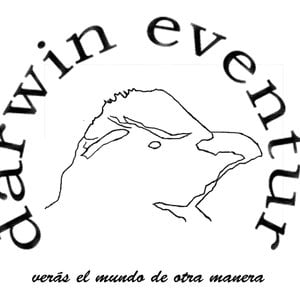
\includegraphics[width=8cm]{./figuras/logo.jpg}
\end{center}
\end{figure}

FACULTAD DE CIENCIAS\\
\vspace*{0.15in}
DEPARTAMENTO DE BIOLOGÍA ORAL \\
\vspace*{0.6in}
\begin{large}
\textbf{AVANCES EN PATOLOGÍA TUMORAL Y NUEVAS
MOLÉCULAS CON APLICACIÓN EN MEDICINA REGENERATIVA} \\
\end{large}
\vspace*{0.2in}
\begin{Large}

\end{Large}
\vspace*{0.3in}
\begin{large}
A work submitted by Dunja Capitán Sobrino for the Regenerative Biomedicine Master \\
\end{large}
\vspace*{0.3in}
\rule{80mm}{0.1mm}\\
\vspace*{0.1in}
\begin{large}
Supervised by: \\
Virginea de Araujo \\
\end{large}
\end{center}

\end{titlepage}
\title{Trabajo de LaTeX}
\maketitle
\twocolumn[
\begin{@twocolumnfalse}
\begin{abstract}

Las MSCs, son un grupo de células madre adultas originadas a partir de la capa germinal mesodermal.El objetivo de este estudio consiste en inducir la diferenciación de estas MSCs hacia un linaje neuronal mediante la aplicación de un medio específico durante 31 días. Tras 31 días, se llevó a cabo RT-PCR e inmunocitoquímica utilizando marcadores neuronales para verificar la diferenciación neuronal no únicamente por microscopía. 
\end{abstract}

\end{@twocolumnfalse}

]

\section*{Introduction}

\lettrine{L}as células estromales mesenquimales multipotentes (MSCs), son un grupo de células madre adultas originadas a partir de la capa germinal mesodermal. Las MSC pueden aislarse de diferentes tejidos incluyendo, entre otros: periostio, médula ósea , grasa, líquido amniótico, folículo piloso, dermis, sangre de cordón umbilical y dientes. Fueron descritas por Friedenstein en 1974. En este ensayo, aislaron células madre adultas no hematopoyéticas de la médula ósea y las definieron como células adherentes de morfología fibroblastoide (Figura 1) con la capacidad de diferenciarse a tejidos mesodérmicos funcionales como osteoblastos, condroblastos y adipocitos. Varios estudios han nombrado a este grupo celular como: Células de Estroma Medular, Unidades Formadoras de Colonias Fibroblastoides, Precursores Estromales o Células Adultas Progenitoras Multipotentes o MAPCs (Multi-Potent Adult Progenitor Cells). Fue en 2006, cuando la Sociedad Internacional de Terapia Celular (ISCT) publicó un informe en el que declaró que “células estromales mesenquimales multipotentes” es la designación actualmente recomendada. Además, la ISCT propuso tres criterios para clasificar una célula como MSC; primero, éstas células deben ser adherentes en cultivo; segundo, expresar los  antigenos CD73, CD90 y CD105 en ausencia de antígenos hematopoyéticos como CD34, CD45, marcadores de monocitos, macrófagos y linfocitos B; y tercero, las MSCs deben ser capaces de diferenciarse in vitro en osteoblastos, adipocitos y condrocitos.En cuanto a su multipotencialidad, varios estudios demuestran que estas células son capaces de transdiferenciarse y generar linajes celulares diferentes de los mesodermales, demostrando así su multipotencialidad expandida. Se ha observado diferenciación de MSCs en células del estroma de la médula, células de grasa, células osteoblásticas, condrocitos, tendinocitos, miocitos, hepatocitos, islotes pancreáticos y neuronas.
Muchos informes han indicado que las MSCs tienen la capacidad de migrar a una lesión tisular (“homing”) mediante varios estímulos presentes en su entorno como factores de crecimiento y factores quimiotácticos. 

\newpage
\begin{tabular}{|c|c|}
\hline 
\multicolumn{2}{|c|}{Medio Neuronal NEU1} \\ 
\hline 
DMEM-HG & 44,6 ml \\ 
\hline 
EFG & 1 ml \\ 
\hline 
LIF & 0,01 ml \\ 
\hline 
bFGF & 0,02 ml \\ 
\hline 
\end{tabular} 





\begin{@twocolumnfalse}
\section*{Fórmulas}

\begin{equation}
\phi = \oint_s \vec{E} \cdot d\vec{S} = \frac{q_{enc}}{\varepsilon_0} \quad \textrm {(Ley de Gauss)} 
\end{equation}
\begin{equation}
\oint_S \vec{B} \cdot d\vec{S} = 0 \quad \textrm {(Ley de Gauss para el campo magnético)} 
\end{equation}
\begin{equation}
\oint_C \vec{E} \cdot \vec{dl} = - \frac{d}{dt} \int_s \vec{B} \cdot d\vec{S} \quad \textrm {(Ley de Faraday)} 
\end{equation}
\begin{equation}
\oint_C \vec{B}\cdot d\vec{l} =\mu_0 \int_S \vec{j} \cdot d\vec{S} + \mu_0 \epsilon_0 \frac{d}{dt0} \int_S \vec{E} \cdot d\vec{S} \quad \textrm {(Ley de Ampére)} 
\end{equation}

\end{@twocolumnfalse}
\begin{figure}[htb]
\begin{center}
\includegraphics[width=8cm]{./figuras/ABSC1.jpg}
\caption{UCSSC T8}
\end{center}
\end{figure}

\afterpage{\newpage}
\newpage
\twocolumn[
\begin{@twocolumnfalse}


\bibliographystyle{acm}
	\bibliography{Readinglist}
En esta sección se va a hablar en la bibliografía. En este caso vamos a hablar de los artículos \cite{Livak2001} y \cite{Racz2014}.


\end{@twocolumnfalse}
]

\afterpage{\null\newpage}

\end{document}